\chapter{Experiment}

\section{Goal of the Experiment}
The main purpose of the experiment is to show that Reinforcement Learning from visual input is possible using Vizia Environment. 	
Additionally, the eperiments tries to check influence of frame skipping on learning process.

\subsection{Experiment's Design}
Experiment consists of testing agents on `basic' scenario that use different \emph{skiprate}. We define \emph{skiprate} as number of game frames that are skiped (ignored) by agent. Skipping a frame is acomplished with makeAction method  (see TODO /REF/) so rewards are acummulated and chosen action is extended for the skipped frames. Skiprate values of 0,1,2,3,4,5,6 and 7 are included in the experiment. 

For each skiprate, agent is to play for epochs. Each epoch requires performing 5000 learning steps, each involving making an action and running a learning update. After the learning portion of each epoch, 100 random test episodes are conducted and mean score is used for assessment.  

\section{Tested Agent's Design}
	The agent is heavily inspired by Google DeepMind Atari DQN \cite{mnih-dqn-2015}\cite{mnih-atari-2013} and is conceptually identical to DeepMind's algorithm. Game is modelled as Markov Decision Process and Q-learning\cite{watkins:mlj92} is used to reach the optimal policy. $\epsilon$-greedy policy with linear $\epsilon$ decay is used to choose actions. Additionally, a technique called experience replay\cite{mnih-dqn-2015} was applied. A convolutional Neural Network is used for approximation of q-values and it is trained with Backpropagation Algorithm\cite{lecun-98b} using Stochastic Gradient Descent with mini-batches. Agent is written in Python and uses Theano\cite{Bastien-Theano-2012}\cite{bergstra+al:2010-scipy} and Lasagne\cite{sander_dieleman_2015_27878} to implement neural networks.

\section{Experimental Setup} 
	\subsection{Operating System and Hardware}
	\begin{description}
		\item[Operating System] Linux Mint 17 x86\_64, kernel 3.13.0-24-generic
		\item[CPU] Intel Core i7-4790, 4x4GHz
		\item[GPU] GeForce GTX 970, 1664 CUDA cores, 4GB RAM
	\end{description}

	\subsection{Game Settings}
		The experiment uses the simplest scenario from the pool, that is the `basic' scenario (see \ref{subsec:basic}). Screen buffer consists of 3 channels (RGB) and resolution is 60x45 pixels.

	\subsection{Neural Network Architecture}
		Network architecture used for the experiment is rather small though it is suspected that it is still excesively robust for such a simple problem. The network consists of two convolutional layers with 32 square filters (7 and 4 pixels wide) each connected to a max-pooling layer with poolsize equal to 2 and rectifiers. Convolutional layers are followed by a fully connected layer with 800 leaky rectified linear units and output layer with 8 linear units coresponding to 8 available actions (combinations of 3 available buttons). 
	
	\subsection{Agent Parameters}
		\begin{itemize}
		\item $\gamma$ (discount factor) = 0.99
		\item learning rate = 0.01
		\item mini-batch size = 40
		\item initial $\epsilon$ = 1.0
		\item final $\epsilon$ = 0.1
		\item steps after which $\epsilon$ decay will start = 100000
		\item steps to fully decrease $\epsilon$ = 100000
		\item replay memory  capacity = 10000
		\end{itemize}
	

\section{Results}
	\subsection{Numerical Issues}
		In case of 0 skiprate a major numerical problem was euncountered. Estimated q-values very rapidly grew to to infinite vallues (in the first epoch) which prevented further learning. Quite unexpectedly, increasing resolution from 60x45 to 120x90 eliminated the problem at the cost of longer learning time. A faulty code is an obvious explenation, however none has been found yet therefore a conceptually oriented mechanism should be also considered. It is suggested that combination of 0 skiprate and low resolution may produce state transitions that incorporate barely distinguishible states. As a consequence each update would signifficantly infaltes q-values for each state and rapidly reach infinities.

		Because high number of epochs required to get fairly satisfying results with skiprate 0, learning was continued to see if it would follow the trend as expected. //TODO

	\subsection{Learning Quality}
		As seen in the Figure \ref{fig:results} all agents reached estimated maximum average score of ~80 or showed trend towards achieving this value. Watching agents play the scenario proved that agents in fact behave very reasonably. They move towards the target and shoot when it appears in front of them. Occasionally agents fire marginally too soon or stay idle (first available action) throughout whole episode. 

	\subsection{Skiprate} 
		As seen in the Figure \ref{fig:results} higher skiprate lead to quicker and smoother learning, which was expected as higher skiprate makes consequences of actions more immediate and easier to notice. It was also anticipated that higher skiprate would slightly lower scores due to lack of so small-grained control. As seen in Table \ref{tab:results} just the oposite is true and it is doubtful that too short training was the culprit since most of agents reach signifficant stability in 80 epochs and do not appear to be able to ever transcend current highscores.  //TODO (more prone to crazy behaviors)
	\begin{table}
		\begin{center}
			\begin{tabular}{ |l || c | r |}
				\hline
				Skiprate & Best epoch score & Mean of 10 best epochs \\ \hline
				0 & 74.17 & 72.679 \\ \hline
				1 & 77.84 & 76.187 \\ \hline
				2 & 79.35 & 77.914 \\ \hline
				3 & 80.98 & 78.695 \\ \hline
				4 & 81.8 & 80.755 \\ \hline
				5 & 81.32 & 80.162 \\ \hline
				7 & 81.08 & 80.496 \\ \hline
			\end{tabular}
		\end{center}
		\caption{Influence of skiprate on achieved highscores.}\label{tab:results}
	\end{table}

	\begin{figure}
		\centering
		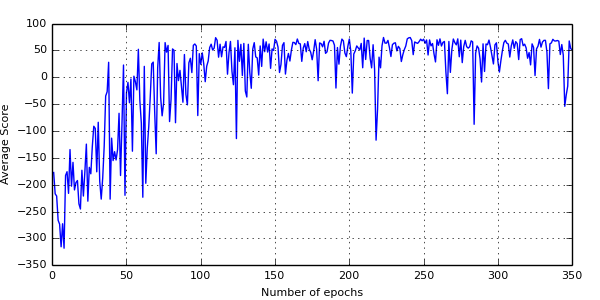
\includegraphics{results_skiprate0.png}
		\caption{Graphs showing mean performance of agent with zero skiprate throughout 350 learning epochs.}\label{fig:results_skiprate0}
	\end{figure}

	\begin{figure}
		\centering
		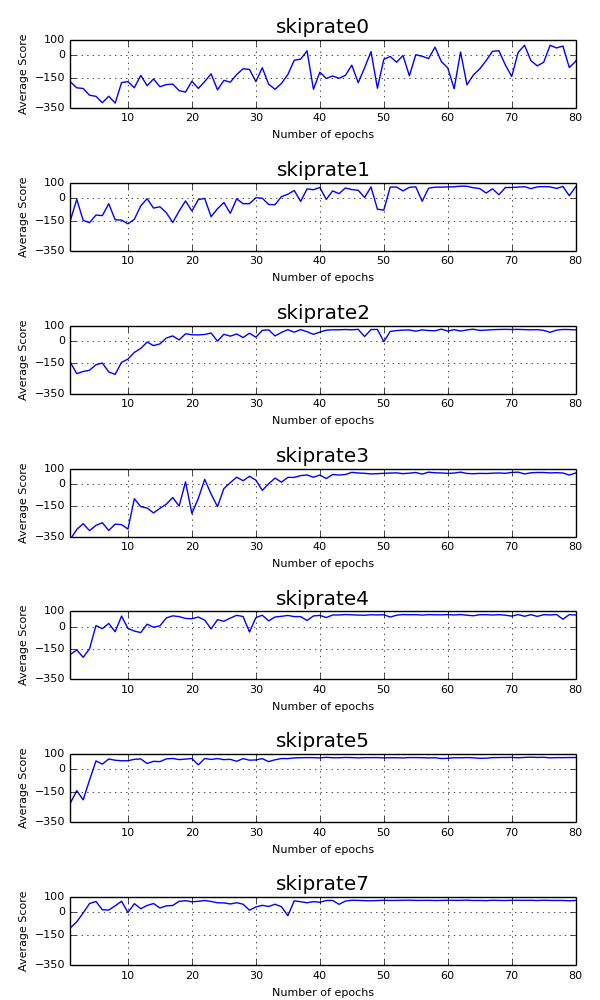
\includegraphics{results.png}
		\caption{Graphs showing mean performance of tested agent with different skip values throughout 80 learning epochs.}\label{fig:results}
	\end{figure}